\documentclass[12pt,openright,oneside,chapter=TITLE,section=TITLE,
    %subsection=TITLE,
    %subsubsection=TITLE,
    brazil]{utfpr-pg}

\renewcommand{\rmdefault}{phv} % Arial
\renewcommand{\sfdefault}{phv} % Arial
\newcolumntype{C}[1]{>{\centering\let\newline\\\arraybackslash\hspace{0pt}}m{#1}}

\usepackage{cmap}
\usepackage[T1]{fontenc}
\usepackage{graphicx}
\usepackage{latexsym}
\usepackage{amssymb}
\usepackage{multirow}
\usepackage{pdfpages}
\usepackage{caption}
\usepackage{scrextend}
\usepackage{forest}
\usepackage{tikz-qtree}


\graphicspath{{./imagens/}}

%Ambiente para gráficos
\DeclareFloatingEnvironment[
fileext=grf,
placement=tbhp,
listname=Lista de Gráficos,
name=Gráfico]{grafico}

\DeclareFloatingEnvironment[
fileext=lod,
listname=Lista de Definições,
name=Definição,
placement=tbhp,
]{definicao}

\setitemize[0]{leftmargin=1.9cm,itemindent=0cm}
\setenumerate[0]{leftmargin=1.9cm,itemindent=0cm}


\departamento{Instituto de Computação}
\curso{Mestrado em Ciência da Computação}
\autor{Breno Leite \\ RA - 192863}
\titulo{A criação de um algoritmo híbrido para a multiplicação de cadeias de matrizes utilizando OpenMP e CUDA}
\tipotrabalho{Projeto final}
\local{Campinas}
\data{2017}
          

% informações do PDF
\makeatletter
\hypersetup{
  % pagebackref=true,
  pdftitle={\@title},
  pdfauthor={\@author},
  pdfsubject={\imprimirpreambulo},
  pdfcreator={LaTeX with abnTeX2},
  colorlinks=false,
}
\makeatother


% Controle do espaçamento entre um parágrafo e outro:
\setlength{\parskip}{0.1cm}  % tente também \onelineskip

\makeindex
\begin{document}
% Retira espaço extra obsoleto entre as frases.
\frenchspacing

\imprimircapa



\textual
\pagestyle{simple}

\chapter{Introdução}
\vspace{-0.7cm}

Muitos problemas na área da computação e matemática utilizam de alguma forma a multiplicação de matrizes. Temos exemplos dentro da álgebra, como as cadeias de Markov, onde uma determinada cadeia pode representar probabilidades de mudanças entre estados de um determinado objeto em um período de tempo \cite{santos2002curso}. A multiplicação de matrizes também é muitas vezes utilizada para a solução de sistemas lineares, dentre outras inúmeras utilidades no meio científico.

O grande problema é que a multiplicação dessa cadeia de matrizes pode ser muito cara computacionalmente, por esse motivo este trabalho tem como intuito apresentar técnicas de paralelização para multiplicar cadeias de matrizes. Neste trabalho serão utilizados paradigmas de programação paralela, juntamente com ferramentas como OpenMP e CUDA para a criação de um algoritmo paralelo híbrido para resolver o problema de multiplicação de cadeias.

\vspace{1cm}
{\let\clearpage\relax \chapter{O problema}}
\vspace{-0.7cm}

Como o custo computacional de multiplicar cadeias de matrizes é normalmente elevado, tem-se um esforço para descobrir métodos mais eficazes de fazê-lo. Sabe-se que a multiplicação de duas matrizes $A_{(n \times r)}$ e $B_{(r \times m)}$ gera uma matriz $C_{(n \times m)}$, onde $n$ e $m$ são as dimensões da nova matriz. O número de operações necessárias para multiplicar as matrizes $A_{(n \times r)}$ e $B_{(r \times m)}$ é dado pela equação $n.m.r$, portanto, é totalmente dependente da dimensão das mesmas. 

A multiplicação de matrizes é uma operação associativa, ou seja, as matrizes $A \ B \ C$ podem ser multiplicadas em ordens diferentes e mesmo assim obter o mesmo resultado. Existe uma ordem de multiplicação das matrizes de tal forma que o número de operações escalares de multiplicação é mínimo. A Tabela \ref{tab:mult} mostra um exemplo de diferenciação na ordem utilizando a seguinte cadeia de matrizes: $A_{(5 \times 2)} \ B_{(2 \times 2)} \ C_{(2 \times 2)}$.

\begin{table}[h]	
	\centering	
	\begin{tabular}{|c|c|} \hline
		\textbf{Parentização} & \textbf{Custo}      \\ \hline
		$((A B) \ C)$             & $5.2.2 + 5.2.2 = 40$  \\ \hline
		$(A \ (B C))$             & $5.2.2 + 2.2.2 = 28$  \\ \hline
	\end{tabular}

	\caption{Diferentes parentizações e seus custos em operações escalares.}
	\vspace{-0.35cm}
	\label{tab:mult}
\end{table}

Podemos perceber que a parentização $(A \ (B C))$ possui o custo mínimo de operações escalares. A diferença entre o mínimo e os outros resultados pode ser muito significante quando o número de matrizes da cadeia cresce. Devido a isto, encontrar a melhor parentização é uma tarefa muito importante na multiplicação de cadeias de matrizes. 

Neste trabalho iremos paralelizar um algoritmo que utiliza conceitos de programação dinâmica para encontrar a melhor parentização para uma determinada cadeia de matrizes, este algoritmo é explicado no capítulo 15.2 do livro do Cormen \cite{cormen2009introduction}. O mesmo tem complexidade de tempo $O(n^3)$, onde $n$ é o número de matrizes de uma determinada cadeia. 

Além de encontrar a melhor cadeia, este trabalho também tem como objetivo multiplicar as matrizes da cadeia de forma paralela. Esse processo não é tão complexo, porém tem um alto custo de memória.

\vspace{1cm}
{\let\clearpage\relax \chapter{Paralelização}}
\vspace{-0.7cm}

Este capítulo tem como objetivo demostrar quais técnicas de paralelização foram aplicadas, assim como as mesmas foram implementadas. O capítulo será dividido em três partes, onde serão explicados o \emph{profiling}, a paralelização para encontrar a melhor parentização e a paralelização da multiplicação da cadeia de matrizes.

\vspace{0.5cm}
\section{Profiling}
\vspace{-0.7cm}

Para o \emph{profiling} do programa foi utilizado a ferramenta \emph{gprof}, o \emph{profiling} do algoritmo serial não foi uma tarefa muito difícil pois o código é bem pequeno e fácil de encontrar os \emph{HotSpots}. 

O importante do \emph{profile} foi notar que dependendo do número de matrizes e suas dimensões o algoritmo podia ter um \emph{HotSpot} diferente, ou seja, quando havia um grande número de matrizes o tempo gasto para encontrar a melhor parentização era o maior. Já quando o número de matrizes era pequeno e as dimensões das mesmas eram grandes, o tempo de multiplicar a cadeia de matrizes era o mais longo.

Outro fato importante percebido é que para entradas com o número de matrizes e dimensões  similares o custo de multiplicar as matrizes é maior, o motivo disto é o alto número de \emph{cache misses} na multiplicação das matrizes. Neste trabalho não vamos nos preocupar com esse problema, mas já existem diversos estudos no meio cientifico relatando esse problema, assim como propondo soluções \cite{lam1991cache}. Uma solução simples é utilizar a matriz transposta no momento da multiplicação, porém, o custo para transformar essa matriz também teria que entrar no computo do tempo para verificar o quanto essa forma resolveria o problema. Alguns trabalhos tratam esse problema com o uso de uma \emph{shared memory}, neste trabalho não aplicamos nenhuma dessas técnicas.

Devido a essa dependência do \emph{HotSpot} com a entrada, foi decidido que ambos os processos deviam ser paralelizados. Ou seja, este trabalho trata da paralelização do algoritmo para encontrar a melhor parentização de determinada cadeia de matrizes, assim como a paralelização da reconstrução dessa parentização e sua multiplicação.

\section{Parentização ótima de uma cadeia de matrizes}
\vspace{-0.7cm}

Conceitos de programação dinâmica são utilizados para resolver o problema de encontrar a melhor parentização para determinada cadeia de matrizes, desta forma, uma tabela é construída para encontrar a solução. Essa matriz é preenchida pelas diagonais,onde cada diagonal representa uma parentização diferente para cada item. A Figura \ref{fig:tabelaPerentizacao} mostra um exemplo de uma matriz utilizada na solução do problema.

\begin{figure}[h]
	\centering	
	{%
		\setlength{\fboxsep}{0pt}%
		\setlength{\fboxrule}{1pt}%
		\fbox{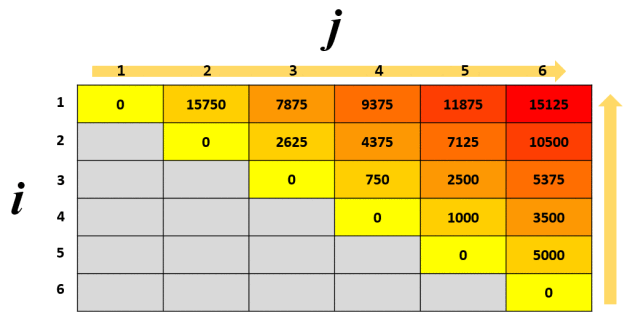
\includegraphics[scale=0.8]{parentizacao.png}}%
	}%
	\vspace{-0.3cm}
	\caption{Matriz de programação dinâmica para o problema} \label{fig:tabelaPerentizacao}
	\vspace{-0.3cm}
	\fonte{\citeonline{Yong}}
\end{figure}

Inicialmente a matriz começa com a sua diagonal preenchida com zeros, e a cada iteração do algoritmo uma nova diagonal é preenchida utilizando dos resultados da diagonal anterior. Mais informações sobre o funcionamento do algoritmo podem ser encontradas no capítulo 15.2 do livro do \citeonline{cormen2009introduction}.

A ferramenta OpenMP foi utilizada para paralelizar este algoritmo, a ideia da paralelização é aproveitar que as diagonais não tem dependência entre sí. Ou seja, o \emph{loop} das diagonais é \emph{DOALL}. Desta forma, cada diagonal é processada em paralelo iterativamente.

 É interessante notar que o número de elementos em cada diagonal diminui em cada interação, o próprio OpenMP toma conta deste ajuste quando chamado dividindo o número de elementos do \emph{loop} pelo número de \emph{threads} utilizadas. Assim que o algoritmo começa uma \emph{pool} de \emph{threads} é criada e para cada iteração do algoritmo os elementos são divididos entre as \emph{threads}. Essa \emph{pool} tem como intuito reduzir o \emph{overhead} de criar \emph{threads} a cada iteração.


\section{Multiplicação de cadeia de matrizes}
\vspace{-0.7cm}

A parelização desta parte do problema foi feita utilizando CUDA, o motivo desta escolha é que algoritmos em CUDA para multiplicação de matrizes são amplamente conhecidos. Porém, apesar de existir diversos algoritmos para multiplicar matrizes em CUDA, a grande maioria deles são projetados para multiplicar duas matrizes e não uma cadeia de matrizes. 

Neste trabalho além da multiplicação da matriz ser paralela, a multiplicação de toda a cadeia de matrizes também é feita em paralelo. Isso significa que encontrada uma melhor cadeia da seguinte forma $((AB)(CD))$ a multiplicação das matrizes $AB$ é feita em paralelo com a multiplicação das matrizes $CD$.

Cada uma das multiplicações é feita em um \emph{kernel} CUDA, e esse mesmo \emph{kernel} é chamado em várias vezes em sequência para todas as matrizes que não tem dependência de outros resultados. Os \emph{kernels} utilizam blocos de $16 \times 16$ e o número \emph{threads} de cada bloco depende da dimensão da matrizes. Essa configuração foi utiliza pois foi a mais comum encontrada na literatura. Além de que essas configurações são boas para a GPU que foi utilizada para os teste, que foi a NVIDIA Kepler K40 do servidor parsusy.

A forma com que duas matrizes são multiplicadas utilizando CUDA é trivial e não vai ser explicada neste trabalho, mais informações sobre esse processo podem ser vistas em \citeonline{Hochberg}.

A dependência entre as multiplicações das matrizes pode ser representada por uma árvore, a Figura \ref{fig:arvore} mostra um exemplo desta árvore para a seguinte cadeia: $(A(BC)(DE))$.

\begin{figure}[h]
	\centering	
	{%	
		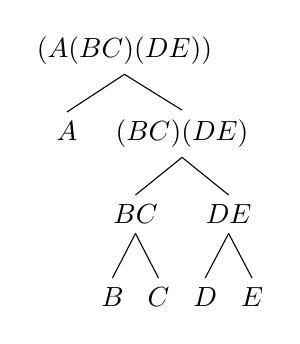
\begin{tikzpicture}
		\Tree [.$(A(BC)(DE))$
		[.$A$ ]
		[.$(BC)(DE)$ 
		[.$BC$ [.$B$ ] [.$C$ ] ] 
		[.$DE$ [.$D$ ] [.$E$ ] ] ]
		]
		\end{tikzpicture}
	}%
	\vspace{-0.3cm}
	\caption{Árvore de dependências} \label{fig:arvore}
\end{figure}

O algoritmo executa essa árvore da direita para a esquerda e das folhas para a raiz.  Para cada nível da árvore $n$ \emph{kernels} CUDA são chamados, e então o algoritmo aguarda todos eles serem resolvidos para passar para o próximo nível da árvore. 

Cada matriz é copiada apenas uma vez para a GPU, a única resposta que é copiada de volta para a CPU é a resposta final. Ou seja, no exemplo da Figura \ref{fig:arvore} as matrizes $D$ e $E$ são copiadas para a GPU, mas a matriz $DE$ não é copiada de volta para a CPU, apenas o resultado final $(A(BC)(DE))$ é copiado de volta para a CPU quando o último nível da árvore é atingido.

\vspace{1cm}
{\let\clearpage\relax \chapter{Metodologia}}
\vspace{-0.7cm}

Este capítulo tem como intuito mostrar a metodologia para os testes feitos neste trabalho, explicando as entradas utilizadas e as formas com que os mesmos foram analisados durante o desenvolvimento do trabalho.

Primeiramente a Tabela \ref{tab:input} define os arquivos de entrada que foram utilizados para os testes. 

\begin{table}[h]	
	\centering
	\resizebox{\textwidth}{!}{%
	\begin{tabular}{|c|c|c|c|c|c|}
		\hline
		\textbf{Arquivo} & \textbf{Nº de matrizes} & \textbf{Dim das matrizes} & \textbf{Arquivo} & \textbf{Nº de matrizes} & \textbf{Dim das matrizes} \\ \hline
		arq1.in          & 1000                        & 50 - 100                       & arq4.in          & 500                         & 50 - 100                       \\ \hline
		arq2.in          & 2000                        & 50 - 100                       & arq5.in          & 500                         & 100 - 150                      \\ \hline
		arq3.in          & 3000                        & 50 - 100                       & arq6.in          & 500                         & 150 - 200                      \\ \hline
		\multicolumn{3}{|c|}{\textbf{Grupo 1}}                                          & \multicolumn{3}{c|}{\textbf{Grupo 2}}                                           \\ \hline
	\end{tabular}
	}
	\vspace{-0.35cm}
	\caption{Descrição dos arquivos de entrada utilizados nos testes.}
	\label{tab:input}
\end{table}

Os arquivos foram divididos em dois grupos, o Grupo 1 são arquivos onde o número de matrizes da cadeia é variado, enquanto as dimensões das matrizes variam entre 50 e 100. Já o Grupo 2 mantém o número de matrizes e varia as dimensões das matrizes, nota-se que a dimensão exata das matrizes são geradas aleatoriamente e 50-100 significa que a matriz de menor dimensão tem 50 e a de maior tem 100.

Esses arquivos serão testados de três formas diferentes, uma comparando somente o \emph{speedup} em relação a encontrar a melhor parentização. Outra levando em consideração que já temos a melhor parentização e comparando o resultado apenas da multiplicação da cadeia, e por ultimo a junção de ambos em um mesmo algoritmo. 

Para os testes serão utilizados 2, 4 e 8 \emph{threads}, é importante perceber que o número de \emph{threads} não influencia no algoritmo de multiplicação da cadeia, o mesmo influência apenas no algoritmo de encontrar a melhor parentização. 

Todos os tempos foram adquiridos utilizando o servidor parsusy, obtendo uma média de 10 execuções para cada caso de teste.

\vspace{1cm}
{\let\clearpage\relax \chapter{Resultados}}
\vspace{-0.7cm}

Este capítulo tem como objetivo mostrar os resultados obtidos com o algoritmo paralelo criado neste trabalho.

\vspace{0.5cm}
\section{Parentização ótima de uma cadeia de matrizes}
\vspace{-0.7cm}

Nesta seção será mostrado os resultados da parte do algoritmo que é responsável em encontrar a melhor parentização possível para determinada cadeia de matrizes. Ou seja, esta seção analisa exclusivamente como o OpenMP se saiu em relação ao algoritmo serial. A Figura \ref{fig:order} mostra a variação do \emph{SpeedUp} em relação ao número de \emph{threads}.

\begin{figure}[h]
	\centering	
	{%
		\setlength{\fboxsep}{0pt}%
		\setlength{\fboxrule}{1pt}%
		\fbox{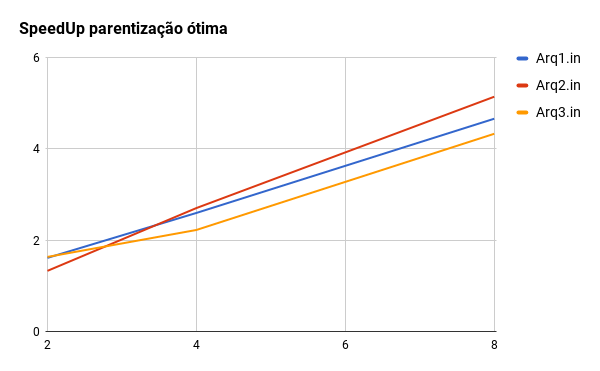
\includegraphics[scale=0.5]{order.png}}%
	}%
	\vspace{-0.3cm}
	\caption{Variação do \emph{SpeedUp} pelo número de \emph{threads}} \label{fig:order}
\end{figure}

A Figura \ref{fig:order} mostra que o algoritmo obteve um resultado de cerca entre 2 e 5 de \emph{SpeedUp}, dependendo da entrada. Percebe-se que o aumento do número de \emph{threads} aumenta o desempenho. Esse aumento continua até 8 \emph{threads}, depois disso o \emph{SpeedUp} atinge seu patamar máximo e começa a reduzir.

Um fato interessante, é que o aumento do número de matrizes não faz com que o \emph{SpeedUp} aumente. Podemos ver no gráfico da Figura \ref{fig:order} que o arquivo 3 teve o menor \emph{SpeedUp}, valores maiores que estes não foram testados por motivos que serão descritos no capítulo relacionado aos problemas encontrados. 

\section{Multiplicação de uma cadeia ótima de matrizes}
\vspace{-0.7cm}

Esta seção tem como objetivo mostrar o desempenho da multiplicação feita na parentização ótima encontrada pelo algoritmo mostrado na seção anterior. Nesta parte vamos comparar apenas os resultados da multiplicação, na próxima seção será analisado o funcionamento dos dois algoritmos em conjunto. A Figura \ref{fig:matrix} faz uma comparação do tempo  em segundos consumido pela GPU para executar a multiplicação utilizando a parentização ótima para as matrizes dos arquivos da Tabela \ref{tab:input}.

\begin{figure}[h]
	\centering	
	{%
		\setlength{\fboxsep}{0pt}%
		\setlength{\fboxrule}{1pt}%
		\fbox{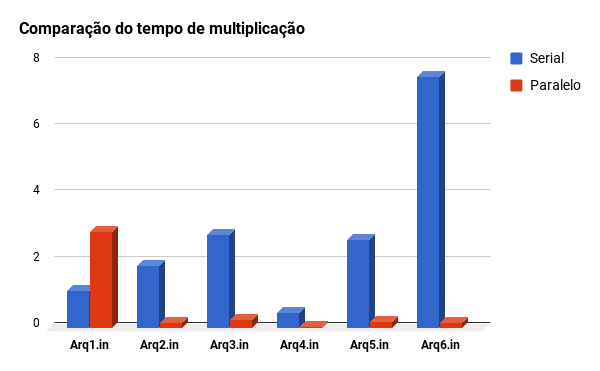
\includegraphics[scale=0.5]{matrix.png}}%
	}%
	\vspace{-0.3cm}
	\caption{Tempo em segundos para multiplicar cadeias dos arquivos} \label{fig:matrix}
\end{figure}

Pode-se perceber para a multiplicação da cadeia o número de matrizes e a dimensão das mesmas tem uma grande influência no tempo de processamento, conforme esse número cresce a tendencia é que o \emph{SpeedUp} cresça. A Tabela \ref{tab:matrix} mostra os \emph{SpeedUp} obtidos pelos tempos mostrados na Figura \ref{fig:matrix}.

\begin{table}[h]	
	\centering
	
	\begin{tabular}{|c|c|c|c|}
		\hline
		\textbf{Arquivo} & \textbf{SpeedUp} & \textbf{Arquivo} & \textbf{SpeedUp} \\ \hline
		arq1.in          & 0.3864           & arq4.in          & 11.9539          \\ \hline
		arq2.in          & 10.7203          & arq5.in          & 14.0967          \\ \hline
		arq3.in          & 10.997           & arq6.in          & 49.3169          \\ \hline
	\end{tabular}
	
	\vspace{-0.35cm}
	\caption{\emph{SpeedUp} multiplicação de cadeias} \label{tab:matrix}
\end{table}

Algo importante de se notar é que o \emph{SpeedUp} entre os arquivos 1 e 4 foram muito diferentes, mesmo com os dois tendo a mesma estrutura de arquivos de entrada. O motivo disto é que a forma que a cadeia está no arquivo 1 é mais difícil de ser multiplicada do que no arquivo 4. O número total de multiplicações foram 273731256  e 134559854 para os arquivos 1 e 4 respectivamente. 

Como a cadeia é mais difícil, o tempo para percorrer a árvore mostrada na Figura \ref{fig:arvore} é maior, o que torna o algoritmo paralelo ruim para o arquivo 1. Esse tempo é irrelevante quando o número de multiplicações necessárias cresce muito.

\section{Algoritmo híbrido OpenMP + CUDA}
\vspace{-0.7cm}

Esta seção irá mostrar os resultados obtidos da junção dos dois algoritmos mostrados anteriormente, a Figura \ref{fig:total} mostra o \emph{SpeedUp} obtido para cada entrada dependendo do número de \emph{threads}.

\begin{figure}[h]
	\centering	
	{%
		\setlength{\fboxsep}{0pt}%
		\setlength{\fboxrule}{1pt}%
		\fbox{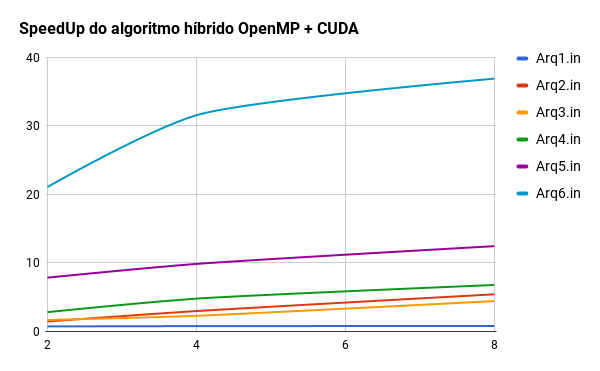
\includegraphics[scale=0.5]{total.png}}%
	}%
	\vspace{-0.3cm}
	\caption{Algoritmo híbrido para multiplicar cadeia de matrizes} \label{fig:total}
\end{figure}

Pode-se perceber que o algoritmo desenvolvido teve um excelente desempenho, dependendo do número de matrizes e da dimensão das mesmas o \emph{SpeedUp} chegou ultrapassar 30 utilizando 8 \emph{threads}.

Percebe-se também que conforme o tamanho do problema aumenta o \emph{SpeedUp} melhora, isso se deve pois o custo do \emph{overhead} é compensado pela solução paralela do problema. Esse aumento é ainda maior quando as dimensões das matrizes são aumentadas, o motivo desta alta melhora é o processamento paralelo tanto da multiplicação dessas matrizes como também a forma com que a parentização e executada em paralelo. Não foi possível verificar até onde esse crescimento acontece, o motivo será explicado no próximo capítulo.

\vspace{1cm}
{\let\clearpage\relax \chapter{Difículdades encontradas no desenvolvimento}}
\vspace{-0.7cm}

A principal dificuldade encontrada foi a alta demanda por memória de acordo com o aumento do tamanho da entrada. Dado os recursos físicos disponíveis para a execução desse software, não pode-se executar testes em escalas maiores., vários métodos tiveram que ser implementados com intuito de economizar e gerenciar melhor a memória disponível. Outro problema foi a falta de um algoritmo serial já implementado, boa parte do algoritmo serial teve que ser implementado pois ambos os problemas são tratados normalmente separadamente.

\vspace{1cm}
{\let\clearpage\relax \chapter{Conclusão}}
\vspace{-0.7cm}

O trabalho mostra um algoritmo híbrido que utiliza conceitos de programação paralela, juntamente com ferramentas como OpenMP e CUDA para otimizar um problema muito conhecido na área científica. O algoritmo criado mostrou-se capaz de obter um \emph{SpeedUp} de quase 40 em determinadas condições, além de ter um bom rendimento no geral. 

A criação do algoritmo foi um processo muito interessante, onde foi envolvido conceitos aprendidos dentro da sala de aula. Assim como uma mistura desses conceitos para resolver um mesmo problema da melhor maneira possível. 

Pode-se perceber também que o número de ferramentas e conceitos aprendidos na disciplina nos proporciona um leque de possibilidades muito útil, e necessário, para resolver problemas que podemos vir a enfrentar no futuro.




\postextual
\bibliography{tcc}

\end{document}
